\section{Jacobian Matrix Compression}
\label{sec:jacobian-matrix-compression}


The main goal of Jacobian matrix compression is minimization of the number of non-linear function evaluations which is quite a computationally intensive operation. Minimization is performed by means of efficient treatment of non-zero entries of a sparse matrix. The problem is also known as matrix partitioning.\\


In the general case, finite difference method can be used to compute a Jacobian matrix approximation in the following way:\\

\begin{equation} \label{eq:matrix-compression-1}
	\frac{1}{\epsilon} (F(y + \epsilon e_{k}) - F(y)) \approx J(y) e_{k}, \: \: \: 1 \leq k \leq N
\end{equation}

where $F : \mathbb{R}^{N} \rightarrow \mathbb{R}^{N}$  is a non-linear function, $e_{k} \in \mathbb{R}^{N}$ is the k\textit{th} coordinate unit vector, $\epsilon$ is a small step size.\\


Equation \ref{eq:matrix-compression-1} does not exploit Jacobian matrix sparsity and, therefore, estimation of a Jacobian matrix requires $N$ function evaluations.\\


\figpointer{\ref{fig:example-of-matrix-compression}}
\begin{figure}[htpb]
  \centering
  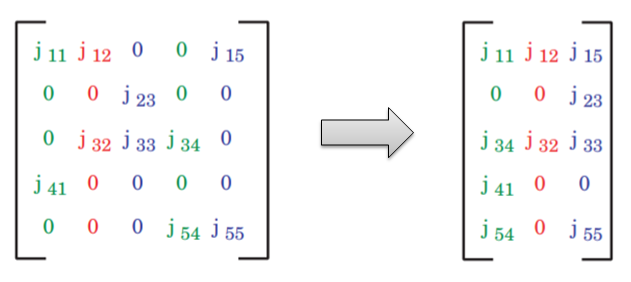
\includegraphics[width=0.55\textwidth]{figures/chapter-3/matrix-compression-example.png}
\caption{An example of matrix coloring and compression \cite{gebremedhin2005color}}
\label{fig:example-of-matrix-compression}
\end{figure}


The compression algorithm is based on the notion of \textit{structurally orthogonal} columns i.e. columns which do not share any non-zero entry in a common row. Figure \ref{fig:example-of-matrix-compression} shows an example of a matrix compression where each color denotes independent \textit{structurally orthogonal} columns.\\


% Curtis, Powell, and Reid [35] were the first to observe in 1974 that sparsity can be employed in this way to reduce the number of function evaluations needed to estimate the Jacobian.


Having obtained a compressed form of Jacobian, another set of vectors $d \in \mathbb{R}^{N}$, also known as seed vectors, can be used to perform function perturbation instead of unit vectors $e_{k}$. A seed vector $d$ has 1’s in components corresponding to the indices of columns in a structurally orthogonal group of columns, and zeros in all other components \cite{gebremedhin2005color}. By differencing the function $F$ along the vector $d$, one can simultaneously determine the nonzero elements in all of these columns through one additional function evaluation at $F(y+d)$ \cite{gebremedhin2005color}.\\


It is obvious the algorithm requires to partition a matrix into the fewest amount of groups, colors, in order to achieve the most of efficiency. There exist various methods and huristics dedicated to that particular problem. \citeauthor{gebremedhin2005color}, in work \cite{gebremedhin2005color}, conducted one of the most recent comprehensive studies in this field and summarized different matrix partitioning algorithms proposed over the last 20 years. Currently, Jacobian matrix compression has been successfully implemented in ATHLET by means of the corresponding built-in PETSc subroutines through NuT interface.\\


% unequal length of MPI messages 
Figure \ref{fig:matrix-partitioning-example} shows an illustrative example of an efficient matrix partitioning where an initial 100 by 100 Jacobian matrix is transformed into its 100 by 28 compressed form using 28 distinct colors. It can be clearly observed from the figure the column vector length of the compressed Jacobian form is gradually decreasing. Figure \ref{fig:matrix-column-distribution} provides a detailed and clear view on the problem, using data from figure \ref{fig:matrix-partitioning-example} as an example, where a bar represents the corresponding column length.\\


\figpointer{\ref{fig:matrix-partitioning-example}}
\begin{figure}[htpb]
  \centering
  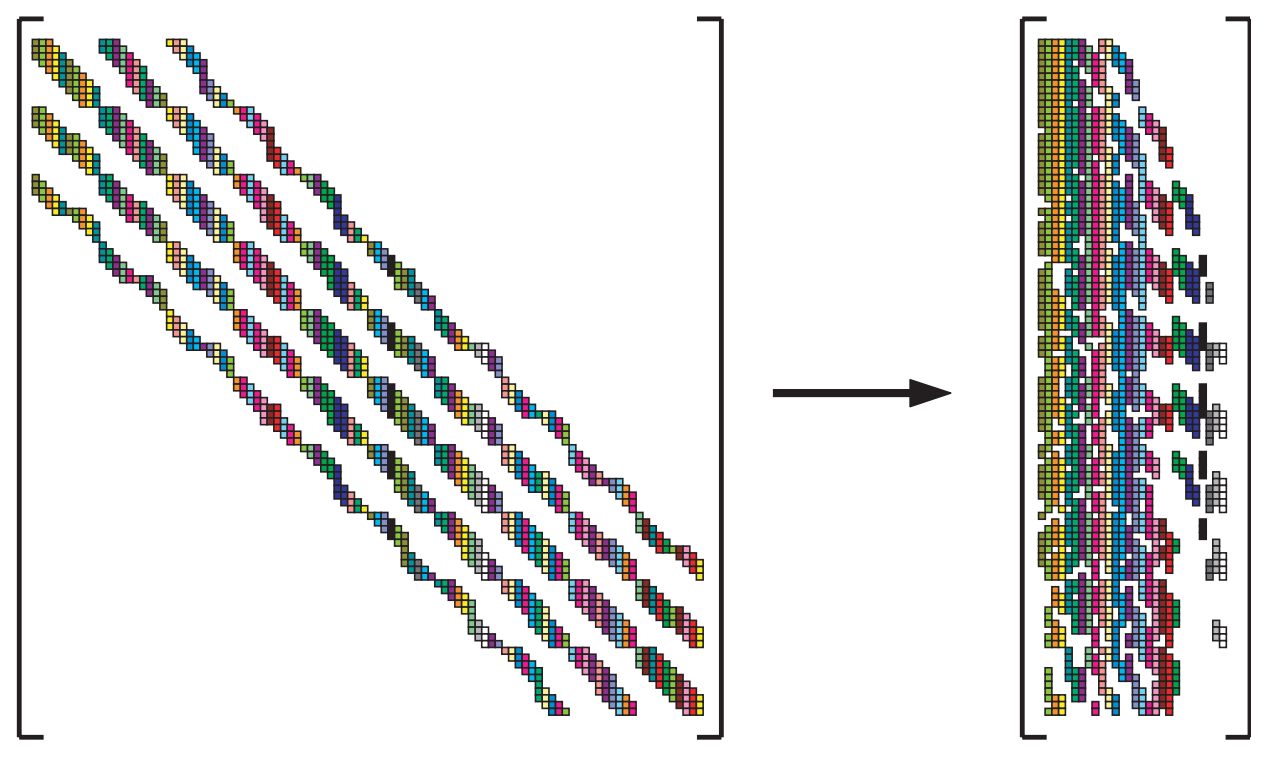
\includegraphics[width=0.8\textwidth]{figures/matrix-compression.png}
  \caption{An example of an efficient Jacobian matrix partitioning \cite{gebremedhin2005color}} \label{fig:matrix-partitioning-example}
\end{figure}


\begin{figure}[htpb]
  \centering
  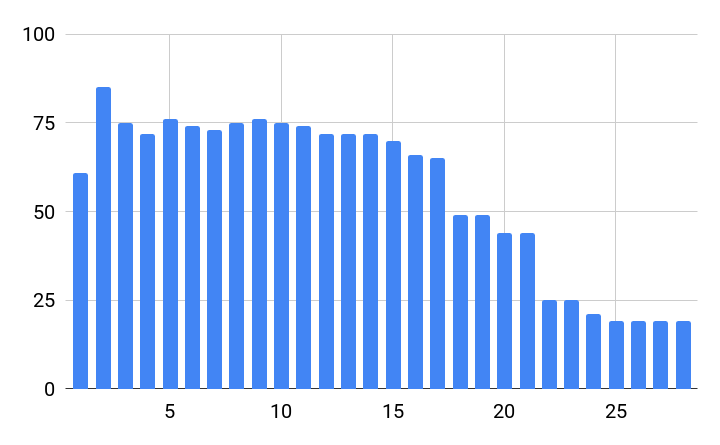
\includegraphics[width=0.7\textwidth]{figures/matrix-compression-2.png}
  \caption{Column length distribution of the example of figure \ref{fig:matrix-partitioning-example}} \label{fig:matrix-column-distribution}
\end{figure}


According to the ATHLET-NuT coupling design, each column is transfered to NuT by means of the synchronous 3-way handshake procedure, described in section \ref{sec:athlet-nut-coupling}, immediately after its evaluation. Thus, the figure \ref{fig:matrix-column-distribution} determines the communication pattern during the Jacobian matrix transfer.\\


% listing
Code listings \ref{lst:athlet-grs-defaul:athlet} and \ref{lst:athlet-grs-defaul:nut} represent the default compressed Jacobian matrix transfer between ATHLET and NuT. This code was used as a baseline for the remaining part of the study.\\


All \textbf{code listings}, presented in this part of the study, are written in \textbf{pseudo-code} and intended for for convenience of reading. The aim is to show and display the main ideas skipping non-relevant parts of the source code. The \textbf{pseudo-code} is a mixture of several programming languages, namely: \textbf{Python}, \textbf{C/C++}, \textbf{Fortran}, \textbf{MPI}.\\


\begin{minipage}{\linewidth}
\begin{lstlisting}[language=python, caption={Pseudocode of the default ATHLET-NuT coupling: ATHLET part}, frame=single, label={lst:athlet-grs-defaul:athlet}]
# GIVEN PARAMETERS:
# acomm - the athlet communicator
# acomm_id - athlet identification number 
# y - known vector
# N - problem size
# COO - compressed matrix coordinate format

eps = 1e-4
center = f(y)
column = zeros(N)

# compute Jacobian and send it to NuT column-by-column
for seed_vector in seed_vectors:

	# compute the next column
	vector = evaluate_jacobian(f, seed_vector, center, eps)
	
	length = perturbed_vector.length
	signal = [encode("add_to_jacobian"), acomm_id]
	
	# perform 3-way handshake
	MPI_Send(signal, 2, int, acomm.head, acomm)
	
	# broadcast jacobian column length
	MPI_Bcast(length, 1, int, acomm.head, acomm)
	
	# broadcast jacobian column
	MPI_Bcast(vector.data, length, COO, acomm.all, acomm)
	

\end{lstlisting}
\end{minipage}



\begin{minipage}{\linewidth}
\begin{lstlisting}[language=python, caption={Pseudocode of the default ATHLET-NuT coupling: NuT part}, frame=single, label={lst:athlet-grs-defaul:nut}]
# N - problem size
# J - allocated distributed jacobian matrix
# COO - compressed matrix coordinate format
nut_running = True

while nut_running:
	if rank in heads:
		
		# receive request
		MPI_Recv(signal, 2, int, NUT_WORLD.any_client, NUT_WORLD)
		
		comm = my_comm_list[signal[1]]
		if (comm not None):
			# posses resources
			MPI_Bcast(signal, 2, int, comm.all, comm)
		else:
			continue
		
	else:
		MPI_Recv(signal, 2, int, NUT_WORLD.any_head, NUT_WORLD)
		
	# decode request
	comm = my_comm_list[signal[1]]
	if (comm not None):	
		request = decode(signal[0])
	
		case(request):
			...
			if (request == "exit"):
				# beak while loop			
				nut_running = False
			
			if (request == "add_to_jacobian"):
				# receive jacobian column length
				MPI_Recv(length, 1, int, comm.client, comm)
	
				# receive row jacobian column
				MPI_Recv(elements, length, COO, comm.client, comm)

			
				for i in range(0, length):
					if (local_min < elements[i].row < local_max):
						J.insert(elements[i])
		...

\end{lstlisting}
\end{minipage}




%The effect of color size reduction is the particularly field of interest in this study because it determines the communication pattern between the client and server. It is well known that sending small messages can lead to performance deterioration due to not full resource utilization. In this case we consider the network bandwidth as the main resource.\\

%\emph{example of jacobian evaluation}


 

% and there exist several algorithms which can tackle it, namely: [reference to the book]

%The coloring technique 